\documentclass[a4paper,10pt]{article}

\usepackage[margin=2cm, tmargin=1.5in, headheight=40px]{geometry}
\usepackage[sfdefault, medium, light]{roboto}
%\usepackage[nomap]{FiraMono}
\usepackage[T1]{fontenc}
\usepackage[utf8]{inputenc}
\usepackage[spanish]{babel}
\usepackage{graphicx}
\usepackage{fancyhdr}
\usepackage{enumitem}
\usepackage{minted}
\usepackage[svgnames]{xcolor}
\setminted{style=default,bgcolor=Gainsboro}
\usepackage[allcolors={DarkSlateBlue}, colorlinks]{hyperref}

\fancyhf{}
\fancyhead[L]{
\includegraphics[height=35px]{../figuras/logoort.png}}
\fancyhead[R]{Facultad de Ingeniería \\ Cátedra de Redes y Sistemas de Comunicación}
\fancyfoot[R]{Página \thepage}
\fancyfoot[L]{Redes -- Laboratorio 5}
\renewcommand{\footrulewidth}{0.2pt}
\renewcommand{\headrulewidth}{0.2pt}

\pagestyle{fancy}


\title{\bf Redes\\Laboratorio 5 -- Capa de Red\\ Ruteo dinámico}
\author{\bf Universidad ORT Uruguay}
\date{\bf Curso 2026}

\begin{document}

\maketitle
\thispagestyle{fancy}


En este laboratorio trabajaremos a nivel de Capa de Red, configurando de forma completa la asignación de direcciones y utilizando el protocolo de \textbf{ruteo dinámico OSPF} buscaremos lograr conectividad a toda la red. En particular los objetivos son:

\begin{itemize}
    \item Realizar una asignación de direcciones de una topología dada.
    \item Configurar dicha asignación en los equipos, tanto routers como hosts, de manera de implementar la capa de red.
    \item Realizar la configuración OSPF para lograr conectividad en toda la topología.
    \item Analizar cómo reacciona OSPF ante cambios de la topología.
\end{itemize}

La práctica puede realizarse de dos maneras:

\begin{enumerate}[label={\bf \alph*)}]
    \item Utilizando los equipos Cisco disponibles en el laboratorio de Redes. Dichos Routers se encuentran pre-cableados en topología de anillo, utilizando enlaces \textbf{seriales} punto a punto. Los routers disponen además de interfaces \textbf{Ethernet} (FastEthernet o GigabitEthernet, según el modelo). Sin embargo, los routers inicialmente tienen todas sus interfaces apagadas y sin configurar (tal como vienen de fábrica). Disponemos de dos anillos de 4 Routers y uno de 3 Routers, así como Switches para implementar las redes locales.
    
    En este caso, cada grupo configurará un único Router, así como los equipos conectados directamente al mismo, poniéndose de acuerdo con los restantes equipos del mismo anillo cuál es la configuración correcta de modo de que la red quede coherentemente configurada.

    \item Utilizando el simulador \href{https://www.gns3.com/}{\bf GNS3} que permite emular en una PC de escritorio una topología de red dada, creando máquinas virtuales que emulan el funcionamiento de los Routers y su sistema operativo. Se proveen en la página del curso archivos de tipo \emph{portable GNS3 project} con topologías similares a las de laboratorio. En este caso, el equipo deberá configurar \emph{toda la topología} para que quede funcionando.
    
\end{enumerate}

\section{Asignación de direcciones}

En esta parte retomamos la asignación de direcciones del Laboratorio 4.

\subsection{Topología de 4 routers}

\begin{figure}
    \begin{center}
    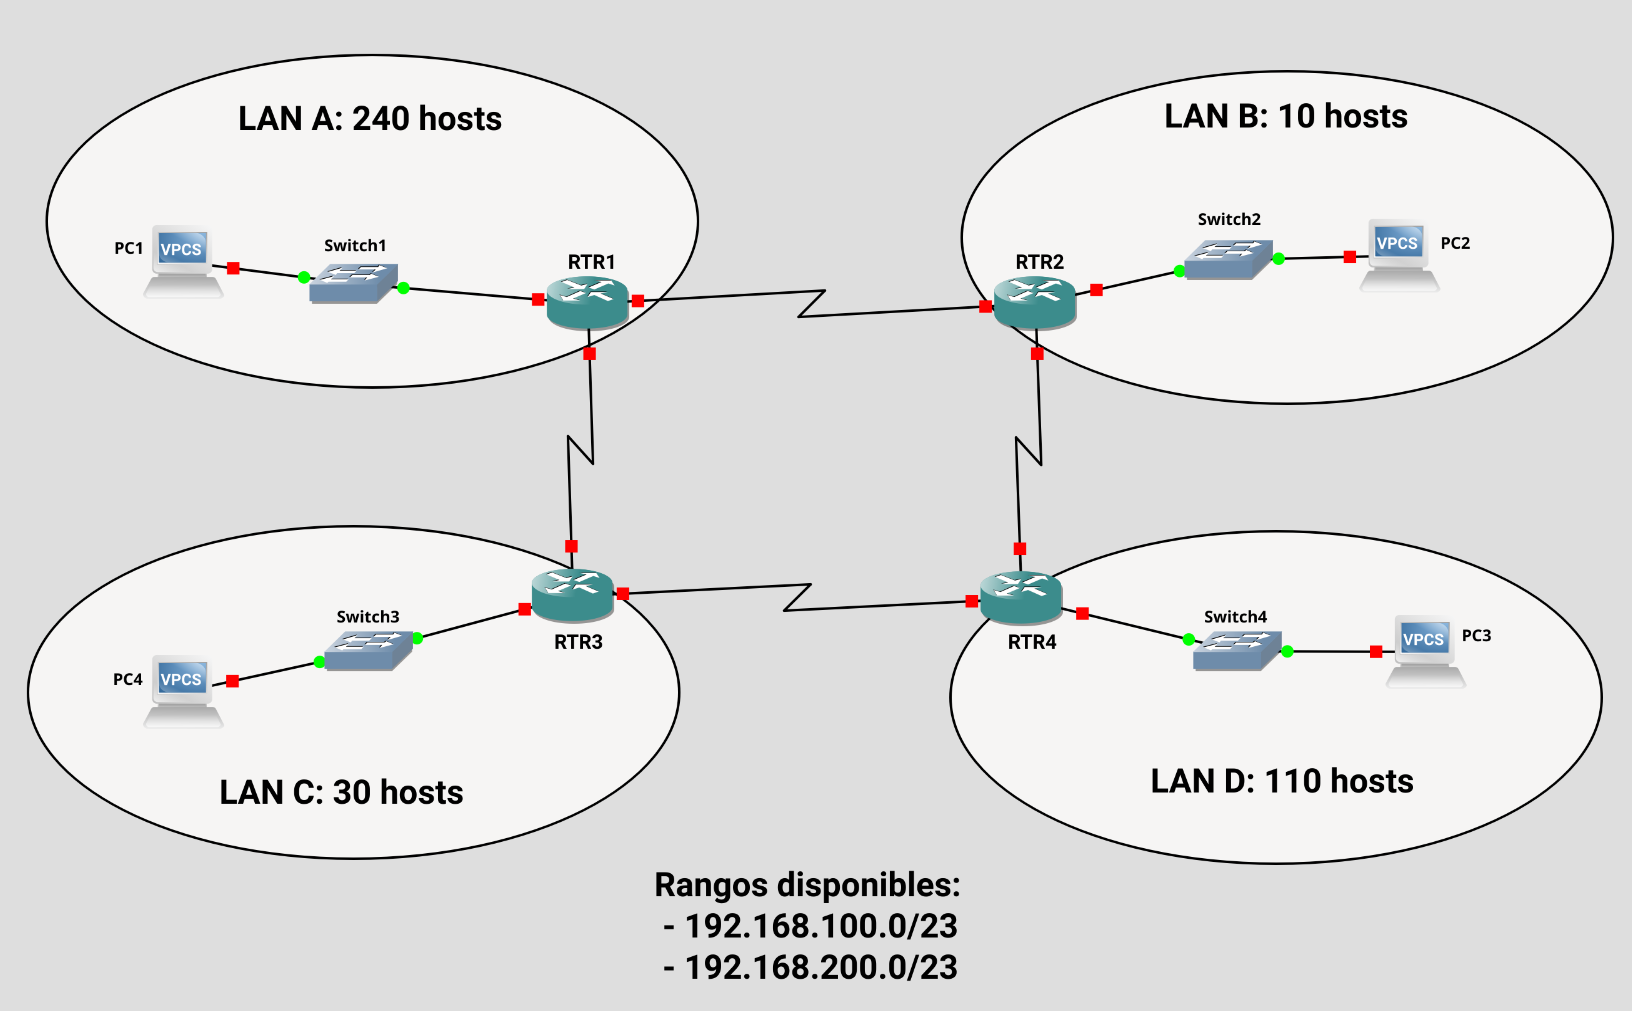
\includegraphics[width=0.95\textwidth]{../figuras/topologia_lab.png}
    \end{center}
    \caption{Topología de Red de 4 routers con rangos a asignar.}\label{fig:topologia}
\end{figure}

Realice una asignación de direcciones completa para las redes de área local de la Figura \ref{fig:topologia}, así como para los enlaces punto a punto entre routers, utilizando el rango provisto. Complete las siguientes tablas

    \begin{center}
        \bigskip
        \begin{tabular}{|p{1cm}|p{3cm}|p{3cm}|p{3cm}|p{3cm}|}
            \hline
            \textbf{Red} & \textbf{Dirección de red} & \textbf{Máscara} & \textbf{Dir. de broadcast} & \textbf{IP Router} \\ \hline
            \textbf{LAN A} & & & & \\ \hline
            \textbf{LAN B} & & & & \\ \hline
            \textbf{LAN C} & & & & \\ \hline
            \textbf{LAN D} & & & & \\ \hline
        \end{tabular}
    \end{center}

    \bigskip
    \begin{center}
        \begin{tabular}{|p{2cm}|p{2.5cm}|p{2.5cm}|p{2.6cm}|p{2.4cm}|p{2.4cm}|}
            \hline
            \textbf{Enlace} & \textbf{Dirección de red} & \textbf{Máscara} & \textbf{Dir. de broadcast} & \textbf{IP Router A} & \textbf{IP Router B} \\ \hline
            \textbf{RTRA--RTRB} & & & & & \\ \hline
            \textbf{RTRA--RTRC} & & & & & \\ \hline
            \textbf{RTRB--RTRD} & & & & & \\ \hline
            \textbf{RTRC--RTRD} & & & & & \\ \hline
        \end{tabular}
    \bigskip
    \end{center}

\subsection{Topología de 3 routers}

    Modifique ahora la asignación anterior para el caso en que hay solo 3 routers, asumiendo que la LAN D y la LAN B son una única LAN con 120 hosts.

        \begin{center}
        \bigskip
        \begin{tabular}{|p{1cm}|p{3cm}|p{3cm}|p{3cm}|p{3cm}|}
            \hline
            \textbf{Red} & \textbf{Dirección de red} & \textbf{Máscara} & \textbf{Dir. de broadcast} & \textbf{IP Router} \\ \hline
            \textbf{LAN A} & & & & \\ \hline
            \textbf{LAN B} & & & & \\ \hline
            \textbf{LAN C} & & & & \\ \hline
        \end{tabular}
    \end{center}

    \bigskip
    \begin{center}
        \begin{tabular}{|p{2cm}|p{2.5cm}|p{2.5cm}|p{2.6cm}|p{2.4cm}|p{2.4cm}|}
            \hline
            \textbf{Enlace} & \textbf{Dirección de red} & \textbf{Máscara} & \textbf{Dir. de broadcast} & \textbf{IP Router A} & \textbf{IP Router B} \\ \hline
            \textbf{RTRA--RTRB} & & & & & \\ \hline
            \textbf{RTRA--RTRC} & & & & & \\ \hline
            \textbf{RTRB--RTRC} & & & & & \\ \hline
        \end{tabular}
    \bigskip
    \end{center}


\textbf{Nota:} antes de continuar, si está trabajando con los equipos del laboratorio, comparta la asignación realizada con el resto de los grupos de su topología de modo de llegar a una asignación coherente. Compare en particular \textbf{cuál es su número de router y cuáles son sus interfaces} con el \textbf{esquema de conexión} disponible en el rack del laboratorio.

\section{Configuración de interfaces}

\begin{enumerate}
    \item Configure cada una de las interfaces de su router, coordinando con los demás routers de su anillo, o bien configure todos los routers en GNS3.
    \item Verifique que:
    \begin{enumerate}
        \item La tabla de ruteo (\mintinline{batch}{RTRX> show ip route}) quedó adecuadamente configurada \emph{solo con las interfaces directamente conectadas}.
        \item Verifique conectividad con los routers vecinos (\mintinline{batch}{RTRX> ping <IP>}).
    \end{enumerate}

\end{enumerate}

\textbf{Nota:} Recuerde que para acceder al router puede utilizar el equipo remotizador de consola disponible en el laboratorio, mediante:
\begin{minted}{batch}
> telnet 172.20.20.24
> Login: grupoX
> Password: ort
\end{minted}
donde X es el no. de router.

En el caso de GNS3, se puede lograr lo mismo con click derecho sobre el router.

\section{Conexión de máquinas de usuario}

\begin{enumerate}
    \item Implemente la red local conectando un Switch a la interfaz Ethernet del router. Verifique que ahora la misma queda activa.
    \item Conecte su máquina del laboratorio a dicha red mediante un patch-cord adecuado, utilizando la tarjeta de red secundaria de la máquina.
    \item Configure la dirección IP, máscara y puerta de enlace predeterminada de su máquina para que quede conectada a la LAN adecuada.
    \item Chequee conectividad con el Router mediante \texttt{ping}. ¿Puede llegar más allá?
\end{enumerate}

Si está trabajando en GNS3, realice los pasos 3 y 4 configurando las PCs virtuales de la topología.

\section{Ruteo dinámico intra-red: OSPF}\label{sec:ospf1}

\begin{enumerate}
    \item Configure OSPF en todos los routers. Asegúrese de que el protocolo quede activo
en todas las interfaces. Utilice el número de área \texttt{0}.

    \item Verifique que el Router logra aprender todos los rangos de su topología. ¿Qué distancia administativa asigna? ¿Qué significa esto? ¿Cuál es la métrica de la ruta?
    
    \item Verifique que ahora puede alcanzar toda la red de su anillo desde cualquier PC.
    
    \item Pruebe cambiar ahora el parámetro \texttt{bandwidth} de una interfaz para ver el efecto en la métrica.
    
    \item Pruebe desconectar una interfaz de un router (quitando el cable o haciendo \texttt{shutdown}). ¿Cuánto demora el protocolo en reaccionar al cambio y recalcular las rutas? ¿Por qué?
    
    \item Pruebe capturar tráfico en el enlace entre la PC y su router. ¿Qué tipo de paquetes OSPF puede ver? ¿Qué rol cumplen?
    
    \item Pruebe cambiar la topología (con \texttt{bandwidth} o bajando una interfaz). ¿Puede ver algún otro tipo de paquete OSPF en la captura? ¿Qué rol cumple? ¿Qué ocurre al reconectar la interfaz?


\end{enumerate}

\appendix

\section{Comandos Cisco}

\textbf{Comandos básicos:}

\begin{itemize}
    \item Ingresar al modo administrador:
\mintinline{batch}{RTRX> enable}
    \item Mostrar la configuración actual: \mintinline{batch}{RTRX# show running-config}
    \item Mostrar las interfaces (resumen): \mintinline{batch}{RTRX# show ip interface brief}
    \item Mostrar la tabla de rutas: \mintinline{batch}{RTRX# show ip route}
    \item Entrar al modo configuración: \mintinline{batch}{RTRX# configure terminal}
    \item Entrar a la conf. de interfaz (ej: FastEthernet 0/0): \mintinline{batch}{RTRX(config)# interface FastEthernet 0/0}
    \item Asignar IP a una interfaz: \mintinline{batch}{RTRX(config-if)# ip address <IP> <mascara>}
    
    donde la IP y la máscara van en formato decimal separadas por puntos.
    \item Encender una interfaz: \mintinline{batch}{RTRX(config-if)# no shutdown}
    \item Asignar IP de broadcast: \mintinline{batch}{RTRX(config-if)# ip broadcast-address <IP>}
    \item Crear una ruta estática: \mintinline{batch}{RTRX(config)# ip route <dir. Red> <máscara> <nextHop>}
    \item Salir de un submenú: \mintinline{batch}{RTRX(config)# exit}

\end{itemize}

\textbf{Comandos OSPF}

\begin{itemize}
    \item Habilitar OSPF \mintinline{batch}{RTRX#(config)> router ospf <num_proceso>}
    \item Agregar redes a la topología OSPF: 
    
    \mintinline{batch}{RTRX(config-router)# network <IP_red> <wildcard> area <num_area>}
    
    Se deben agregar una por una todas las redes en que se desee utilizar. \texttt{wildcard} es el complemento a 1 de la máscara, utilizado por razones históricas. Ejemplo: máscara \texttt{255.255.255.192} $\mapsto$ wildcard \texttt{0.0.0.63}.

    \item Habilitar sumarización por área: \mintinline{batch}{RTRX(config-router)# area <num_area> range <IP_red> <mask>}
    
    Esto debe hacerse sólo en los routers intra-área.

    \item Mostrar información de OSPF: \mintinline{batch}{RTRX# show ip ospf database}
    
    \item Redistribuir rutas de otro protocolo: \mintinline{batch}{RTRX(config-router)# redistribute <protocol> <id>}
    
\end{itemize}


\end{document}